% P05 diagnostic figure reliability_bins|development|M01; allowlisted public aggregate points.
% Each point is an aggregate mean or bin over repeated contexts, not an independent sample.
% data_sha256=7f60e425b5fe235c362c21442c3237e1521aad33df8bebdebfd5854e0cfadd4b
\documentclass[tikz,border=5pt]{standalone}
\ifdefined\pdfinfoomitdate\pdfinfoomitdate=1\fi
\ifdefined\pdfsuppressptexinfo\pdfsuppressptexinfo=-1\fi
\ifdefined\pdftrailerid\pdftrailerid{}\fi
\usepackage{pgfplots}
\usepgfplotslibrary{groupplots}
\pgfplotsset{compat=1.18}
\definecolor{p05Blue}{HTML}{0072B2}
\definecolor{p05Orange}{HTML}{E69F00}
\definecolor{p05Green}{HTML}{009E73}
\definecolor{p05Purple}{HTML}{CC79A7}
\definecolor{p05Red}{HTML}{D55E00}
\definecolor{p05Sky}{HTML}{56B4E9}
\begin{document}
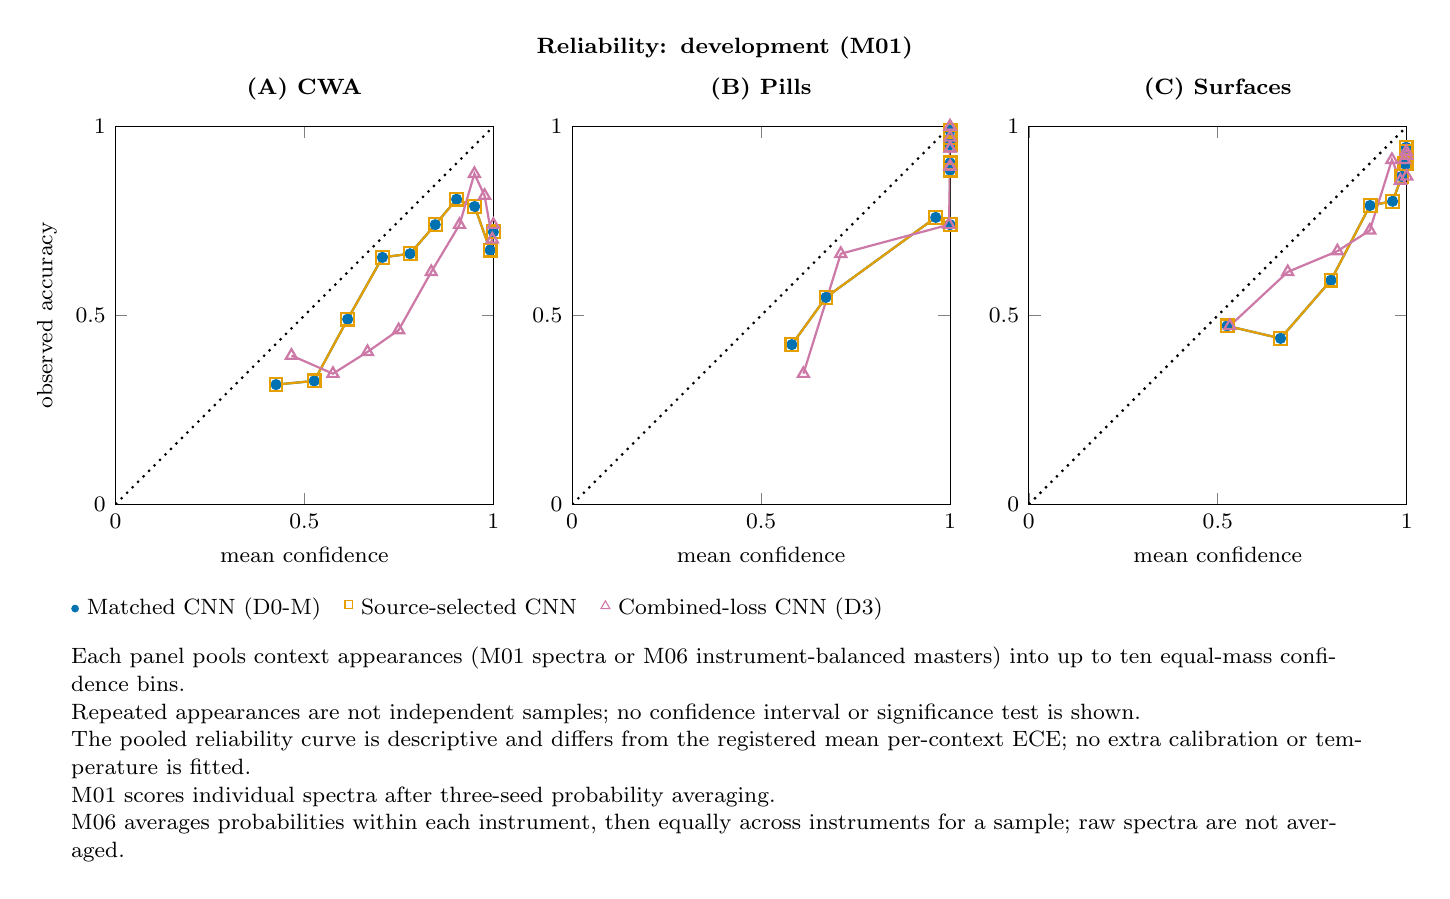
\begin{tikzpicture}
\begin{groupplot}[
  group style={group size=3 by 1, horizontal sep=1.0cm, vertical sep=1.8cm},
  width=4.8cm, height=4.8cm, scale only axis,
  xmin=0, xmax=1, ymin=0, ymax=1,
  xtick={0,0.5,1}, ytick={0,0.5,1},
  tick label style={font=\fontsize{8}{10}\selectfont, color=black},
  label style={font=\fontsize{8}{10}\selectfont, color=black},
  title style={font=\fontsize{8}{10}\selectfont\bfseries, color=black},
]
\nextgroupplot[title={(A) CWA}, xlabel={mean confidence}, ylabel={observed accuracy}]
\addplot[black, dotted, line width=0.8pt] coordinates {(0,0) (1,1)};
\addplot[mark=*, mark size=1.6pt, color=p05Blue, line width=0.8pt, mark options={fill=p05Blue, draw=p05Blue}] coordinates {(0.42495748507698367,0.31730769230769229) (0.52599017065118558,0.32692307692307693) (0.61448306624181659,0.49038461538461536) (0.70641943622639292,0.65384615384615385) (0.77951788565075897,0.66346153846153844) (0.8462238496557124,0.74038461538461542) (0.90258145866804051,0.80769230769230771) (0.9505567633160682,0.78846153846153844) (0.99145759305658465,0.67307692307692313) (0.99996063322819029,0.72115384615384615)};
\addplot[mark=square, mark size=2.3pt, color=p05Orange, line width=0.8pt, mark options={fill=none, draw=p05Orange}] coordinates {(0.42495748507698367,0.31730769230769229) (0.52599017065118558,0.32692307692307693) (0.61448306624181659,0.49038461538461536) (0.70641943622639292,0.65384615384615385) (0.77951788565075897,0.66346153846153844) (0.8462238496557124,0.74038461538461542) (0.90258145866804051,0.80769230769230771) (0.9505567633160682,0.78846153846153844) (0.99145759305658465,0.67307692307692313) (0.99996063322819029,0.72115384615384615)};
\addplot[mark=triangle, mark size=2.3pt, color=p05Purple, line width=0.8pt, mark options={fill=none, draw=p05Purple}] coordinates {(0.46573734689862406,0.39423076923076922) (0.57552304329575743,0.34615384615384615) (0.66695321461708112,0.40384615384615385) (0.74940116565225956,0.46153846153846156) (0.8357080587244311,0.61538461538461542) (0.91049287432404591,0.74038461538461542) (0.94983024781923997,0.875) (0.97671337039498596,0.81730769230769229) (0.99716649859425399,0.70192307692307687) (0.99998385048410643,0.74038461538461542)};
\nextgroupplot[title={(B) Pills}, xlabel={mean confidence}]
\addplot[black, dotted, line width=0.8pt] coordinates {(0,0) (1,1)};
\addplot[mark=*, mark size=1.6pt, color=p05Blue, line width=0.8pt, mark options={fill=p05Blue, draw=p05Blue}] coordinates {(0.58144843201447327,0.42307692307692307) (0.6717022695293321,0.54807692307692313) (0.96209483981310728,0.75961538461538458) (0.99999955693237075,0.74038461538461542) (0.99999999999997935,0.88461538461538458) (1,0.90384615384615385) (1,0.95192307692307687) (1,0.95192307692307687) (1,0.97115384615384615) (1,0.99038461538461542)};
\addplot[mark=square, mark size=2.3pt, color=p05Orange, line width=0.8pt, mark options={fill=none, draw=p05Orange}] coordinates {(0.58144843201447327,0.42307692307692307) (0.6717022695293321,0.54807692307692313) (0.96209483981310728,0.75961538461538458) (0.99999955693237075,0.74038461538461542) (0.99999999999997935,0.88461538461538458) (1,0.90384615384615385) (1,0.95192307692307687) (1,0.95192307692307687) (1,0.97115384615384615) (1,0.99038461538461542)};
\addplot[mark=triangle, mark size=2.3pt, color=p05Purple, line width=0.8pt, mark options={fill=none, draw=p05Purple}] coordinates {(0.61196154518347479,0.34615384615384615) (0.7109644552599228,0.66346153846153844) (0.99720797634254332,0.74038461538461542) (0.99999999897331149,0.89423076923076927) (1,0.89423076923076927) (1,0.94230769230769229) (1,1) (1,0.94230769230769229) (1,0.97115384615384615) (1,1)};
\nextgroupplot[title={(C) Surfaces}, xlabel={mean confidence}]
\addplot[black, dotted, line width=0.8pt] coordinates {(0,0) (1,1)};
\addplot[mark=*, mark size=1.6pt, color=p05Blue, line width=0.8pt, mark options={fill=p05Blue, draw=p05Blue}] coordinates {(0.5246321389352766,0.47252747252747251) (0.66608685219262664,0.43956043956043955) (0.79962446221002181,0.59340659340659341) (0.90285437052415574,0.79120879120879117) (0.96249803244483323,0.80219780219780223) (0.98721419808707478,0.86813186813186816) (0.99522132757996917,0.90109890109890112) (0.99850850135556057,0.94505494505494503) (0.99982076782672458,0.93406593406593408) (0.99999855130846294,0.90109890109890112)};
\addplot[mark=square, mark size=2.3pt, color=p05Orange, line width=0.8pt, mark options={fill=none, draw=p05Orange}] coordinates {(0.5246321389352766,0.47252747252747251) (0.66608685219262664,0.43956043956043955) (0.79962446221002181,0.59340659340659341) (0.90285437052415574,0.79120879120879117) (0.96249803244483323,0.80219780219780223) (0.98721419808707478,0.86813186813186816) (0.99522132757996917,0.90109890109890112) (0.99850850135556057,0.94505494505494503) (0.99982076782672458,0.93406593406593408) (0.99999855130846294,0.90109890109890112)};
\addplot[mark=triangle, mark size=2.3pt, color=p05Purple, line width=0.8pt, mark options={fill=none, draw=p05Purple}] coordinates {(0.53171625592405458,0.47252747252747251) (0.68516451323667726,0.61538461538461542) (0.81647850430085234,0.67032967032967028) (0.90225234313234381,0.72527472527472525) (0.96079498173435585,0.91208791208791207) (0.98323205719879925,0.8571428571428571) (0.99402658279516043,0.91208791208791207) (0.99872534439153871,0.93406593406593408) (0.99990617428790063,0.92307692307692313) (0.99999999886273727,0.86813186813186816)};
\end{groupplot}
\node[anchor=south, font=\fontsize{8}{10}\selectfont\bfseries, color=black, align=center, text width=16.6cm] at (current bounding box.north) {Reliability: development (M01)};
\node[anchor=north, font=\fontsize{8}{10}\selectfont, color=black, align=left, text width=16.6cm] (p05legend) at ([yshift=-2mm]current bounding box.south) {\tikz[baseline=-0.6ex]\fill[p05Blue](0,0)circle(1.4pt);\ Matched CNN (D0-M)\quad \tikz[baseline=-0.6ex]\draw[p05Orange](0,0)rectangle(2.8pt,2.8pt);\ Source-selected CNN\quad \tikz[baseline=-0.6ex]\draw[p05Purple](0,0)--(1.6pt,2.8pt)--(3.2pt,0)--cycle;\ Combined-loss CNN (D3)};
\node[anchor=north, font=\fontsize{8}{10}\selectfont, color=black, align=left, text width=16.6cm] at ([yshift=-1mm]p05legend.south) {Each panel pools context appearances (M01 spectra or M06 instrument-balanced masters) into up to ten equal-mass confidence bins.\\Repeated appearances are not independent samples; no confidence interval or significance test is shown.\\The pooled reliability curve is descriptive and differs from the registered mean per-context ECE; no extra calibration or temperature is fitted.\\M01 scores individual spectra after three-seed probability averaging.\\M06 averages probabilities within each instrument, then equally across instruments for a sample; raw spectra are not averaged.};
\end{tikzpicture}
\end{document}
